\section{Results}
This chapter shows the results of our research methods that we have used.

\subsection{Survey results}
From our survey form, we received 47 results, with all questions completed. We converted the data returned to us to a CSV (Comma-separated values) file and imported it into RStudio, as we did not want the data visualized by Google itself. From our survey we took the questions that we found the most useful and visualized them into plots. 
\begin{figure}[H]
	\centering
	\textbf{\caption{Question: What type of network do you use for playing games?}}
	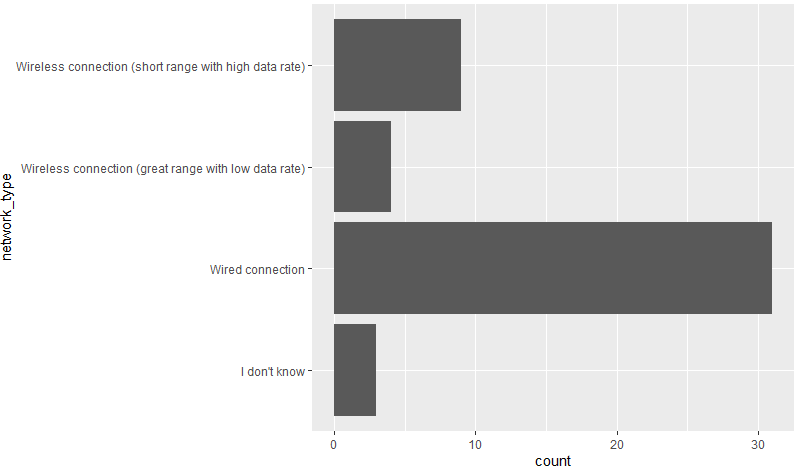
\includegraphics[width=12cm]{../img/network.png}
	
\end{figure}

The barplot shows that most people make use of a wired connection when they play games, where a few people use a wireless connection with either a great range (low data rate) or short range (high data rate). What was alos included in this survey was the question what system the interviewee uses to play video games, the most picked option was Windows/Microsoft. Which makes sense why the wired connection has been picked the most from this question, since wired connection is the most preferred connection type for PC gaming.

\begin{figure}[H]
	\centering
	\textbf{\caption{Question: Do you have a strong internet connection?}}
	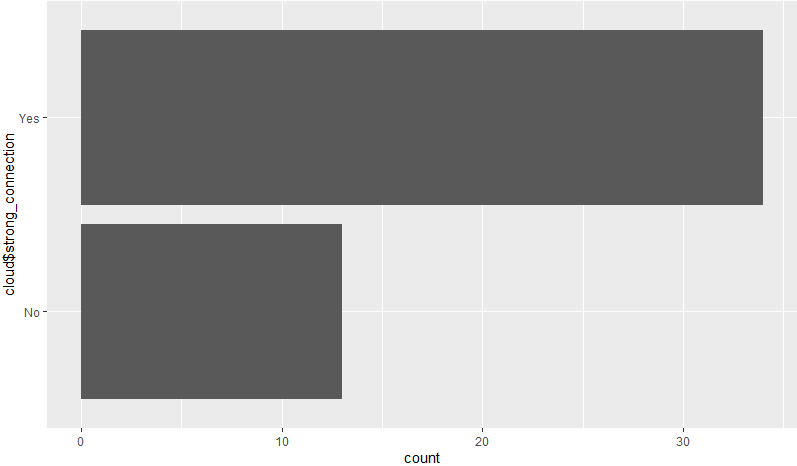
\includegraphics[width=12cm]{../img/connection.png}

\end{figure}

As shown in the chart above, most people claimed that they have a strong Internet connection, while a few people claimed that they do not have a strong Internet connection. We claimed from this that those who had chosen the option "No", that they use a wireless connection and the rest chose the option "Yes" because of a wired connection.

\begin{figure}[H]
	\centering
	\textbf{\caption{Question: When you play an online game, do you often have latency issues?}}
	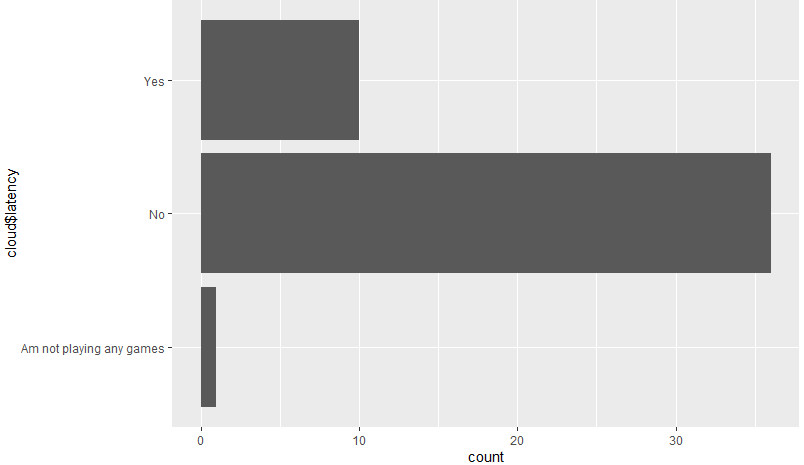
\includegraphics[width=12cm]{../img/latency.png}

\end{figure}

Most people said that they don't often experience latency/lag issues when they play an online game, but a few do experience latency. The people that answered "No" are most likely users of a wired internet connection, whereas the people that have said "Yes" are using a wireless connection.

\begin{figure}[H]
	\centering
	\textbf{\caption{Question: How interested are you in cloud gaming?}}
	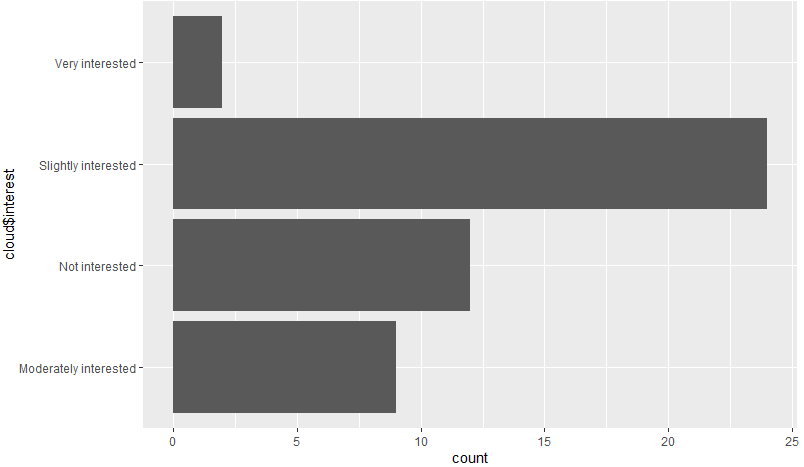
\includegraphics[width=12cm]{../img/interest.png}
	
\end{figure}

People had the choice to fill in how interested they are in cloud gaming. Most people have said that they are slightly interested in it. \\\textbf{From high to low:}\\\\
	Super interested\\
	Very interested\\
	Moderately interested\\
	Slightly interested\\
	Not interested\\\\
In the survey, we also had questions that were about the use of cloud gaming and what the respondents thought of it, such as: For cloud gaming you are attached to a monthly fee between 10 and 60 euros, that in cloud gaming you stream your games from a data center and not at home and that you require a strong and stable internet connection to make the best use of cloud gaming. Most interviewees had mixed thoughts about cloud gaming, which could have affected the question about the interest, having it mixed results. Half of all respondents gave it slight interest and a quarter chose to have no interest in it.

\begin{figure}[H]
	\centering
	\textbf{\caption{Question: Do you think cloud gaming has a future?}}
	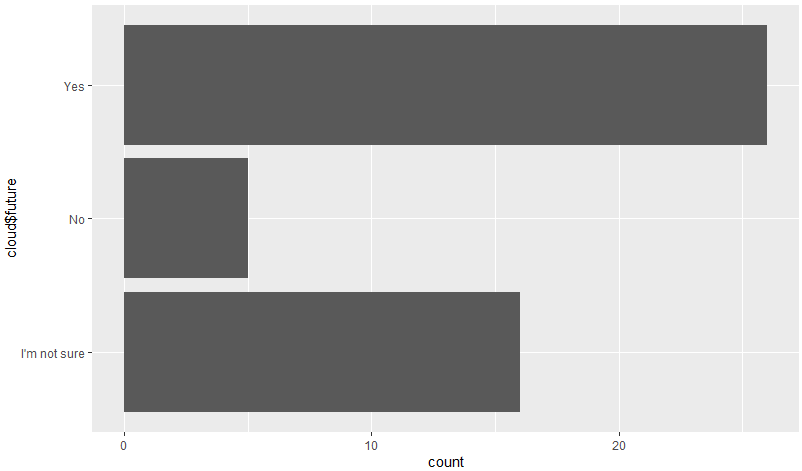
\includegraphics[width=12cm]{../img/future.png}

\end{figure}

For this question, respondents could answer whether cloud gaming has a future for video games. They could choose "Yes", "No" or "I'm not sure". Although there were mixed interests in cloud gaming, many believed that cloud gaming could have a future for video games, in which some did not believe in it, or were unsure about it

\begin{figure}[H]
	\centering
	\textbf{\caption{Question: How likely are you going to give cloud gaming a try?}}
	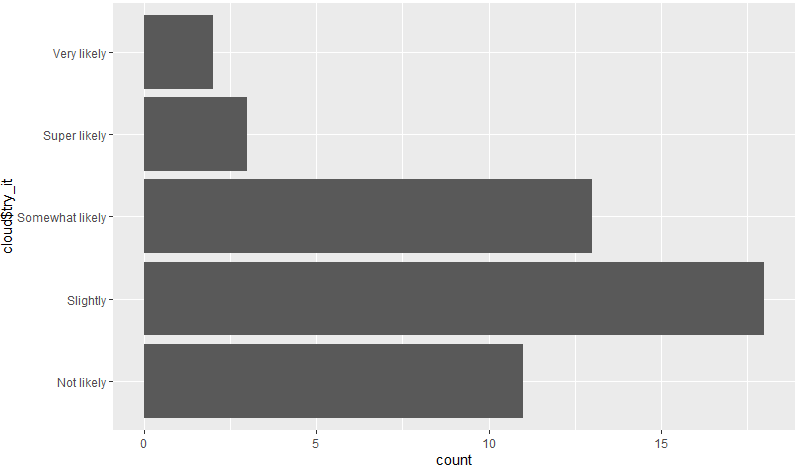
\includegraphics[width=12cm]{../img/try.png}
\end{figure}

Just like the question about how interested people were in cloud gaming, for this question people had the choice to fill in how likely they want to give cloud gaming a try. \\\textbf{From high to low:}\\\\
	Super likely\\
	Very likely\\
	Somewhat likely\\
	Slightly\\
	Not likely\\
	
This question was considered redundant by some interviewees. This could be true because the question about interest in cloud gaming was quite similar, only our thinking on this question was different. We saw this question as literally "Are you ever going to try cloud gaming?", but was changed to "How likely is it that you will try cloud gaming?", and most saw this as an unnecessary question because they had previously indicated whether they were interested in cloud gaming. In which the most frequently chosen option was "Slightly", as with the question about interest.